\chapter{Introduction}


\section{Overview}
\begin{figure}[H] 
	\centering 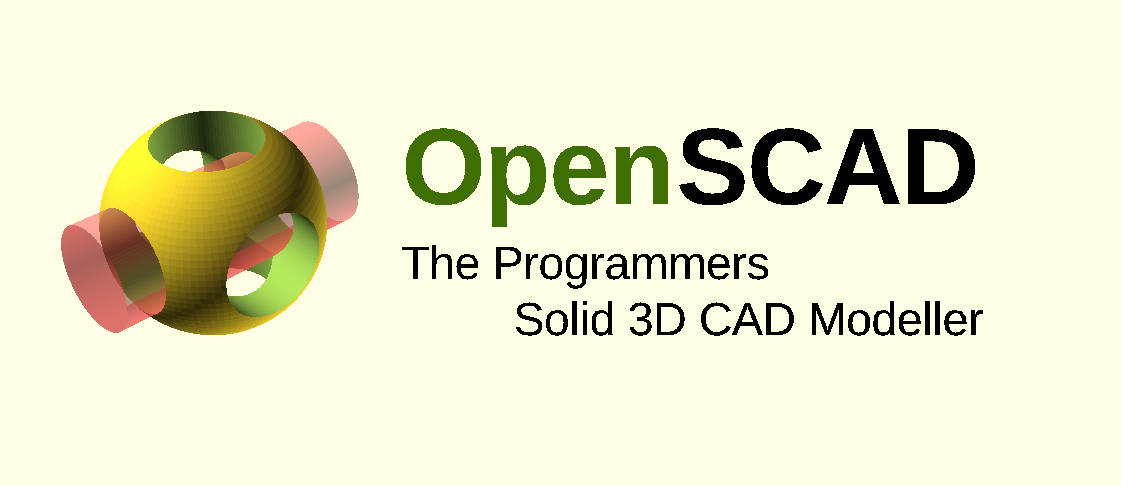
\includegraphics[scale=0.31]{images/openscad.png}
	\caption{OpenSCAD's logo}
	\label{fig:openscadlogo}
\end{figure}
Multi-threaded compile and render for OpenSCAD is our major project. It is under the umbrella organization of BRL-CAD. OpenSCAD is a free and Open-source software application for creating solid 3D CAD objects. It is a script only based modeler, with a specific description language. Parts cannot be selected or modified by mouse in the 3D view. An OpenSCAD script specifies geometric primitives and defines how they are modified and manipulated to render a 3D model. OpenSCAD is available for Windows, Linux and OS X. It does constructive solid geometry (CSG).

OpenSCAD has in a way redefined how easy 3D modeling can be. But the Wikipedia article on OpenSCAD says that it is a non-interactive modeler, but rather a 3D compiler based on a textual description language. Pay attention to the above line, it is primarily what I will be talking about.

Solid 3D modeling. That sounds like some serious business. But it's just an awesome tool for making models pertaining to many uses (mostly 3D printing). And 3D printing as we can all agree upon is cool. 3D models can be created by anyone using OpenSCAD. OpenSCAD is as much for designers as it is for you and me. What else can most people agree upon apart from the fact that solid 3D modeling is cool? A graphical interface is simpler and more intuitive to use. There is a general aversion for typing commands in order to get things done. Simply put, more people have an inclination towards GUI. Another concern is speed at which the results are presented before the user. It would be a waste of CPU capacity if not all of it is being used in the compilation and rendering of the models created in OpenSCAD. This can be achieved by spliting the process into multiple threads.

Since the rendering of various models internally done using the CGAL library, it becomes very important to check how the library behaves on a multi-threaded approach. This is something that will be considered before actually starting the implementation.



\section{Project Category}
OpenSCAD is a free and Open-source software application for creating solid 3D CAD objects. It is under the umbrella organisation of BRL-CAD. Since our project comes under OpenSCAD, it can be classified as being an application development project. But as much as it is an application development project, it is also a research project. It took a fair share of observation and study in order to find the right approach the problem. The majority of the time was spent in figuring out how the internals of this huge piece of software work. The study involved learning about various mathematical constructs used in the geometry of the models. Researching the computer graphics part of the sotware was also very essential in order to form a stronger understanding of how the problem in hand is to be tackled. As mentioned before, the CGAL library (which is used to render the models) is not entirely thread safe. So it bacame very crucial to analyse what parts of it are being used in the render process and how these parts actually work.
Upon researching the above mentioned things, the right way was to be decided upon. The project essentially changes the design approach of an important segament of OpenSCAD i.e. rendering. So of course it required great consideration before implementing it.


\section{Objectives of the Project}
Objective of this project are following:
\begin{itemize}
\item Explore different OS independent ways of parallizing the evaluation.
\item Support for multi-threaded evaluation, possibly with some limitations to handle non-thread-safe library calls
\item Thread safe cache infrastructure
\item Support for safe halting of the render process.
\item Fixing some grammer related oversights in the modelling language.
\item Installing warning mechanism in case of there being multiple pseudo node tags in the model.
\end{itemize}


\section{Problem Formulation}
The following considerations lead to the formation of issues that then transpired into this project:
\begin{itemize}
	\item The rendering process was a bottleneck in performance.
	\item The time it took to render big models really made it cumbersome for the modelers to make small changes and watch their effect as part of their regular testing of the model.
	\item The software was not fully utilizing the cpu cores of the system on which it is run hence the efficeincy as well as time consumption was compromised.
	\item Since the rendering process involves traverssing, processing and then actuating on screen; nodes of an already formed tree; parallel processing the nodes was a clear idea moving forward.
	\item Having separate threads processing separate nodes in the tree was not a straightforward choice because the underlying library as well as the code structure of the software was not thread safe to satisfaction. By this it means that while processing various nodes, the methods used access the same variables in a non safe manner that can be used only in sequential access but will not work right in concurrent access. The same issue is with the CGAL library used in rendering. It also is not ideal for parallel processing.
	\item When the rendering command is given unintentionally then there must be a fault safe method of revoking this command without wipping out the already processed nodes from cache.
	\item The progress bar is not generalised for all kind of structural primitives. This restricts its potency.
	\item When nodes are traverssed in parallel, there is no control over the order in which they are traverssed. As such the progress report code in its current form will not be able to report the progress correctly.
	\item In assigning some nodes as pseudo root for certain renders, the user is not given any warning in case of there being multiple such tags in the description of the model.
	\item There are some oversights in the modelling language that allow for some incomplete syntax to go undetected. This needs to be fixed by improving the grammer.
\end{itemize}
All of the above things lead to the formation of issues that are attempted to be solved in this project.


\section{The Existing System}
OpenSCAD in its present form applies the compile and render process sequentially in one thread of a process. The whole process begins when the user write (or completes) the textual description of their model and chooses to either just compile it or complie and render it one go (F6). The textual description of the language is taken through the following stages sequentially.
\begin{enumerate}
	\item The descriptional language is scanned, tokenized and converted into an Abstract Syntax Tree (AST). This is much like what any compiler does initially.
	\item The AST is converted into an Abstract Node Tree. This consists of the nodes that are to become the part of the final model.
	\item The node tree is fed to the CSGEvaluator which generates a preview of the model abstracting finer details.
	\item The final rendering of the model is done by the GeometryEvaluator.
	\item There are some cases where incorrect use of certain syntax is not caught. This may lead to unexpected behaviour.
	\item When tagging certain nodes as root for the next render, the user is allowed to tag more than one node. In such cases, no warning is given to the user on how this may lead to unexpected behaviour.
	\item The cancel button on the progress report widget does not work for CGAL rendering.
\end{enumerate}

\begin{figure}[H]
\centering
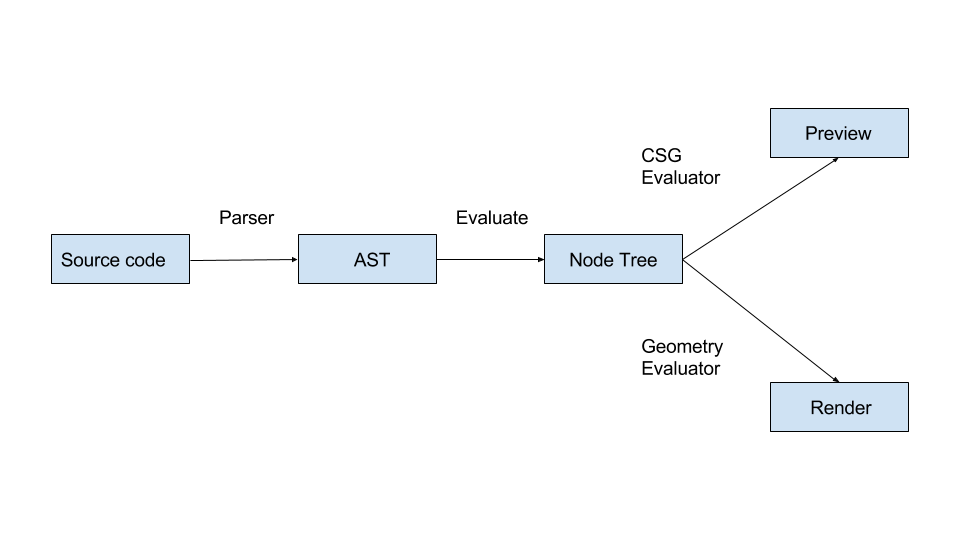
\includegraphics[width=\linewidth]{images/flowchart}
\caption{Present FlowChart}
\label{fig:flowchart}
\end{figure}

The present system is a bit slow in terms of its usage of the available CPU power. In being a single threaded process, everything has to happen in a sequence. This is not something which is required all the time. For example, during the evaluation of the node tree, various nodes can be evaluated in parallel in separate threads. Similarly at the time of rendering, this parallelism can be achieved.

{\bf {Limitations of previous system }}
\begin{itemize}
	\item Not utilizes the full potential of the CPU.
	\item The rendering process is very slow.
	\item When the user accidentely presses F6, there is no way to cancel that process and the user has to wait for the rendering to finish in order to continue their work.
	\item The system hangs frequently for more complex models on normal computers.
	\item It uses large amount of system resources. Their can be a significant improvement in this.
\end{itemize}
